
\section{Results and discussion}\label{sec:discussion}

The results are shown in Figure~\ref{prop-results}. 
The tree models fit the training data well, reaching 98.9, 98.8, and 98.4\% overall accuracy respectively in the $\le$6 setting, with the LSTM underfitting slightly at 94.8\%. 
In that setting, all models generalized well to structures of familiar length, with the tree models all surpassing 97\% on examples of size 4, and the LSTM reaching 94.8\%.
On the longer test sentences, the tree models decayed smoothly in performance across the board, while the LSTM decayed more quickly and more abruptly, with a striking difference in the $\le$4 setting, where LSTM performance falls 10\% from 4 to 5, compared to 4.4\% for the next worse model. However, the LSTM improves considerably with more ample training data in the $\le$6 condition, showing only a 3\% drop and generalization results better than the best model's in the $\le$3 setting.

All four models robustly beat the simple baselines reported in \newcite{Bowman:Potts:Manning:2014}: the most frequent class occurs just over 50\% of the time and a neural bag of words model does reasonably on the shortest examples but falls below 60\% by bin~4.

The learning curve (Figure~\ref{fig:lc}) suggests that additional data is unlikely to change these basic results. The LSTM lags behind the tree models across the curve, but appears to gain accuracy at a similar rate.


\begin{figure*}[t]
  \centering
  \begin{subfigure}[t]{0.04\textwidth}
      
\includegraphics[height=1.25in]{scale.pdf}
\end{subfigure}
\begin{subfigure}[t]{0.24\textwidth}
  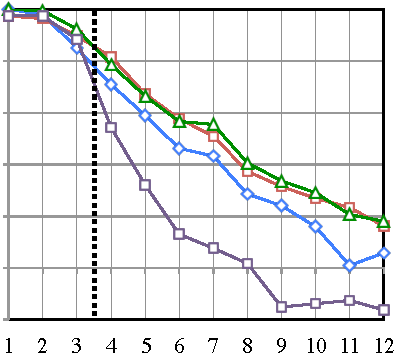
\includegraphics[height=1.25in]{fig3c.pdf}
  \caption{Training on sz. $\le$3.}
  \end{subfigure}~~~
\begin{subfigure}[t]{0.24\textwidth}
    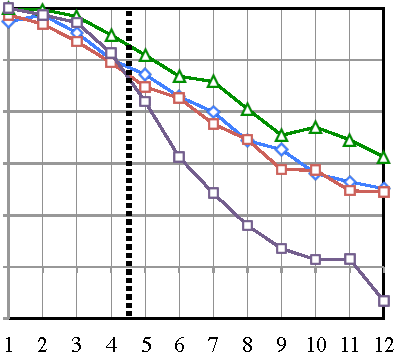
\includegraphics[height=1.25in]{fig4c.pdf}
  \caption{Training on sz. $\le$4.}
  \end{subfigure}~~~
\begin{subfigure}[t]{0.24\textwidth}
      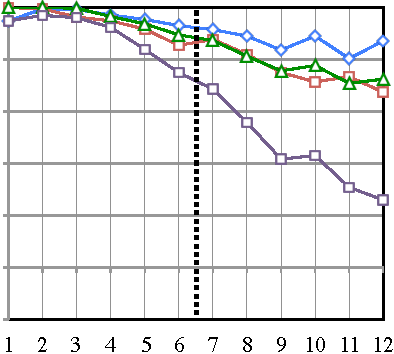
\includegraphics[height=1.25in]{fig6c.pdf}
  \caption{Training on sz. $\le$6.}
\end{subfigure}~~
\begin{subfigure}[t]{0.08\textwidth}
      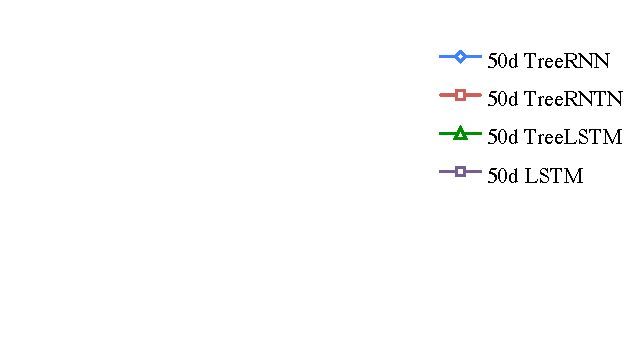
\includegraphics[height=1.25in]{leg.pdf}
\end{subfigure}
  \caption{Test accuracy on three experiments with increasingly rich training sets. The horizontal axis on each graph divides the test set expression pairs into bins by the number of logical operators in the more complex of the two expressions in the pair. The dotted line shows the size of the largest examples in the training set in each experiment.}
  \label{prop-results} 
\end{figure*}

\begin{figure}[t]
  \centering
      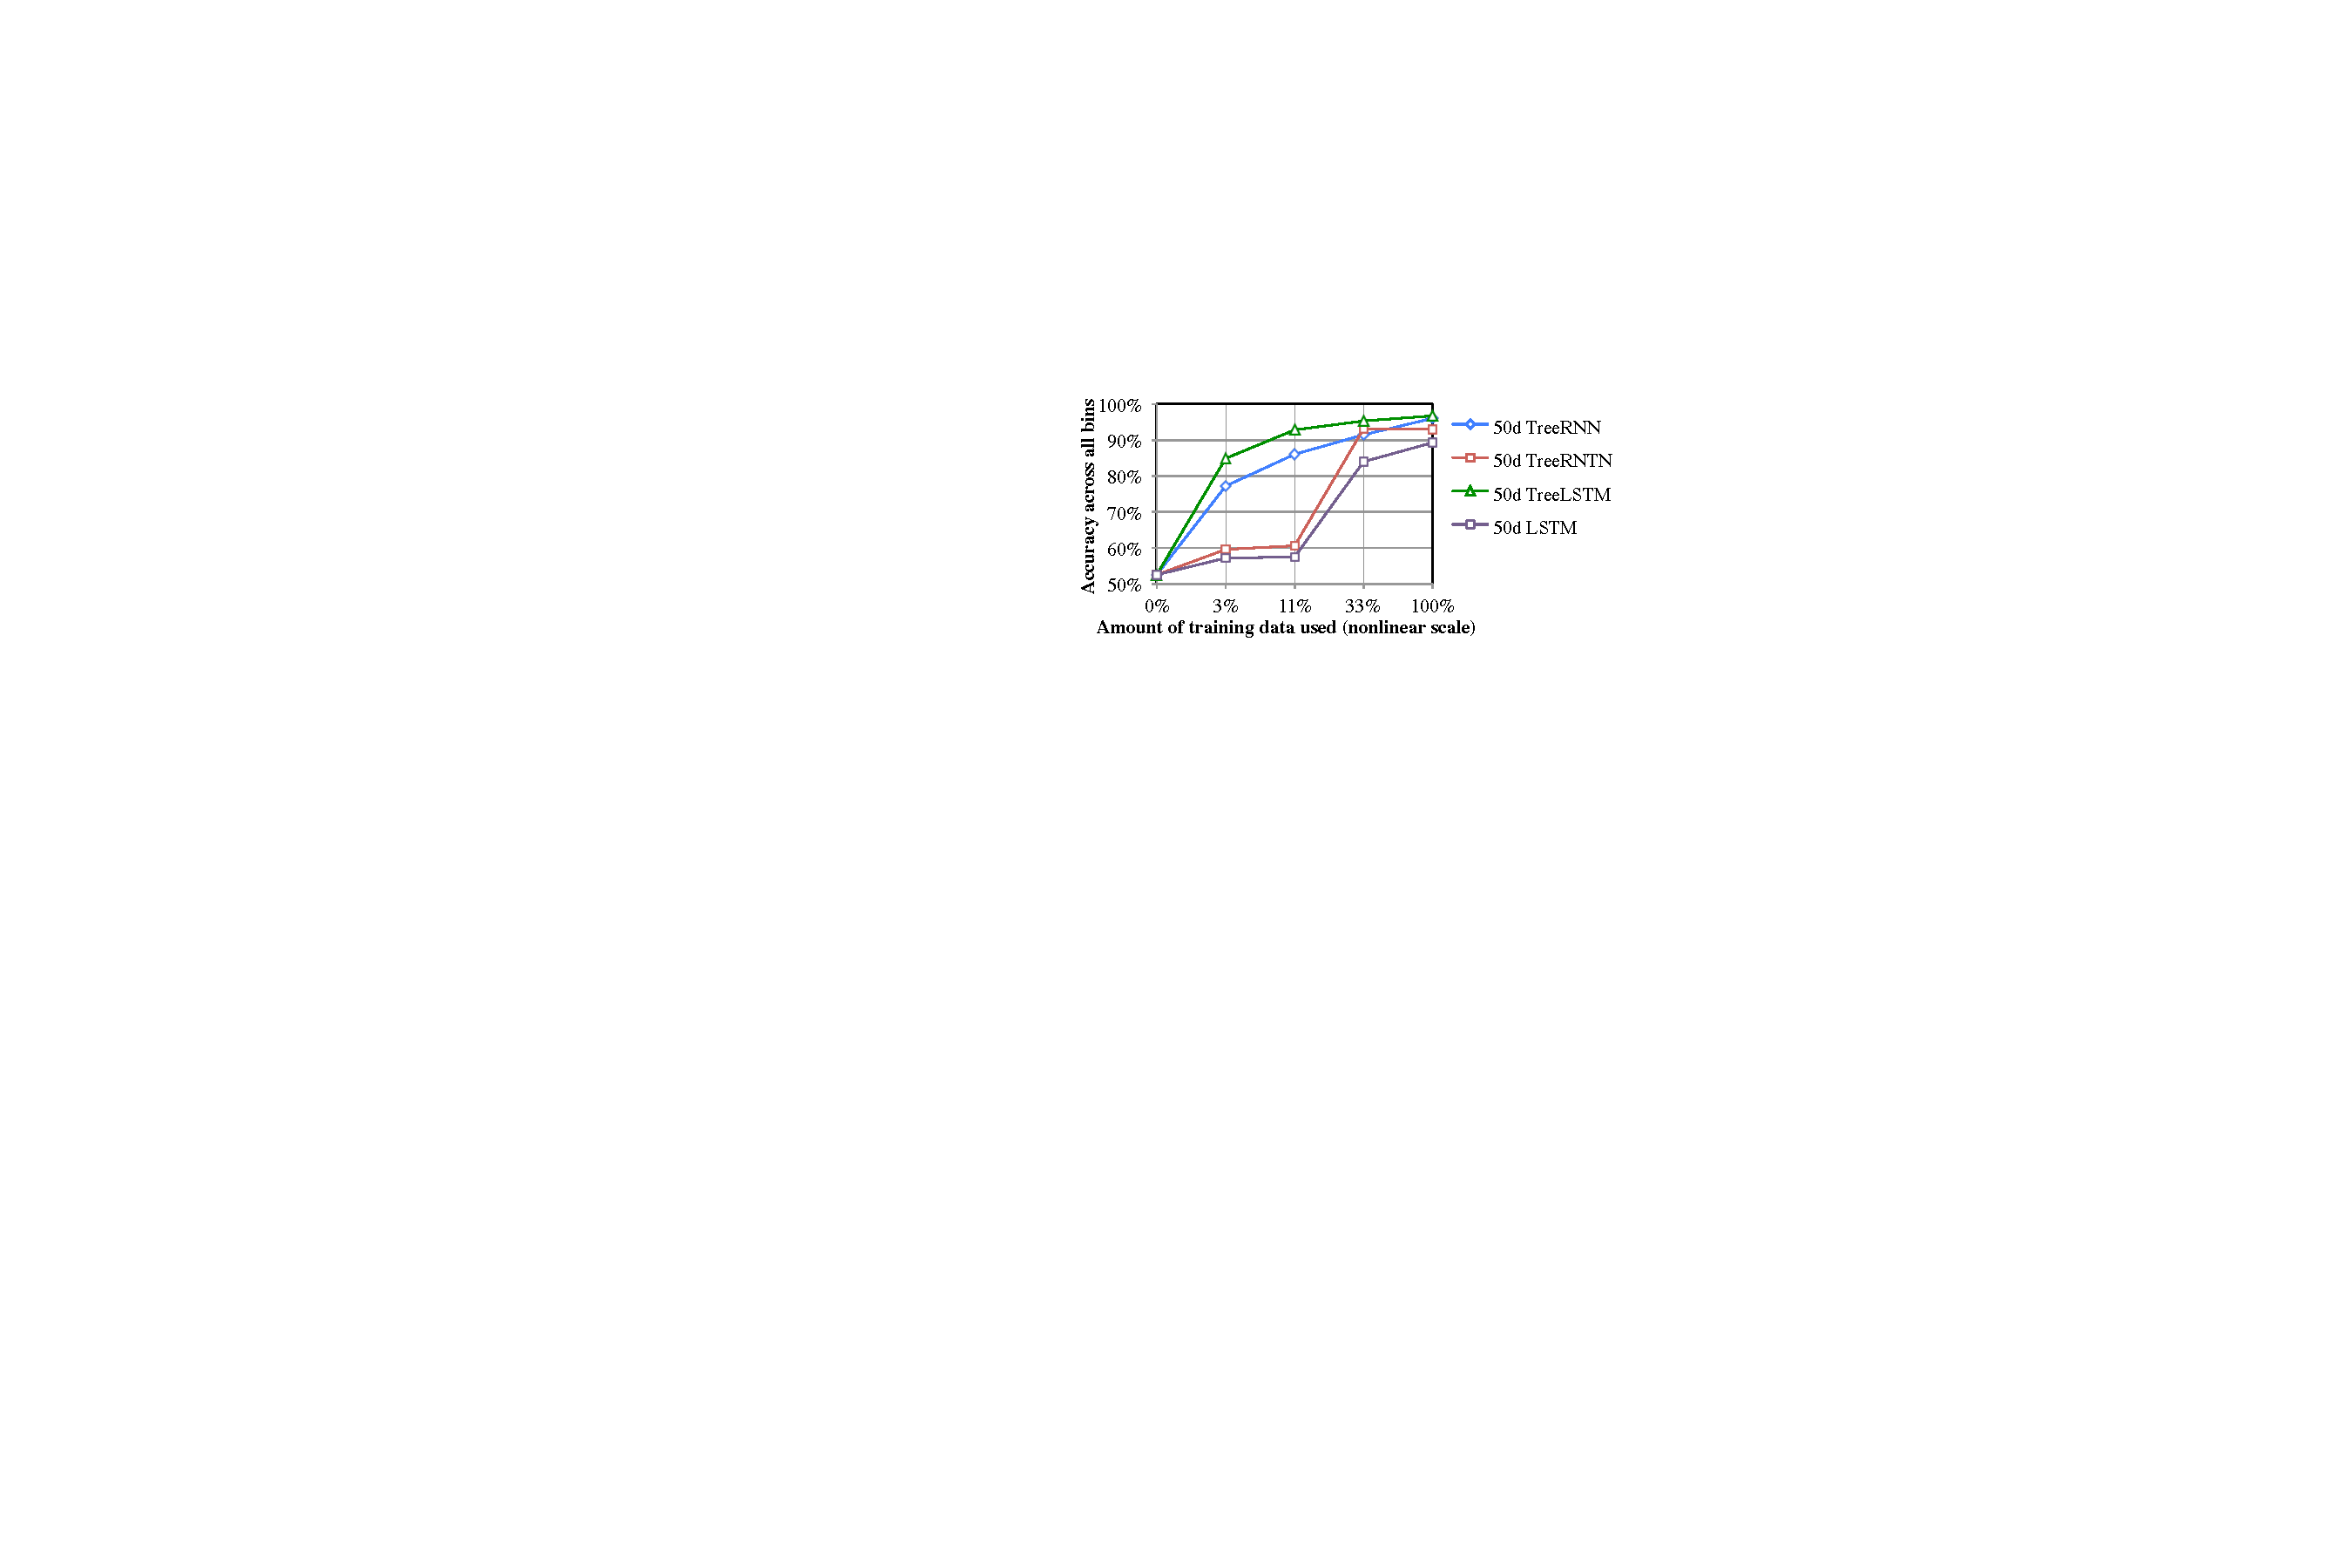
\includegraphics[height=1.1in]{lc.pdf}
  \caption{Learning curve for the $\le$6 experiment.}
  \label{fig:lc} 
\end{figure}


\section{Conclusion}

We found that all four models were able to effectively exploit a recursively defined language to interpret sentences with complex unseen structures.
We find that tree models' biases allow them to do this with greater efficiency, outperforming sequence-based models substantially in every experiment. However, our sequence model was nonetheless able to generalize smoothly to from seen sentence structures to unseen ones, showing that its lack of explicit recursive structure did not prevent it from recognizing recursive structure in our artificial language.

We interpret these results as evidence that both tree and sequence architectures can play valuable roles in the construction of sentence models over data with recursive syntactic structure. Tree architectures provide an explicit bias that makes it possible to efficiently learn to compositional interpretation, which is difficult for sequence models. Sequence models, on the other hand, lack this bias, but have other advantages. Since they use a consistent graph structure across examples, it is easy to accelerate minibatch training in ways that yield substantially faster training times than are possible with tree models, especially with GPUs. In addition, when sequence models integrate each word into a partial sentence representation, they have access to the entire sentence representation up to that point, which may provide valuable cues for the resolution of lexical ambiguity, which is not present in our artificial language, but is a serious concern in natural language text.

Finally, we suggest that, because of the well-supported linguistic claim that the kind of recursive structure that we study here is key to the understanding of real natural languages, there is likely to be value in developing sequence models that can more efficiently exploit this structure without fully sacrificing the flexibility that makes them succeed.
